\section{Method}
\label{sec:method}

\subsection{Problem Formulation}
\label{sec:problem}

We start from a MAML checkpoint with meta-trained initialization $\theta_0$. At meta-test time, a task $\mathcal{T}_i$ provides a support set $S_i=\{(x_k^S,y_k^S)\}_{k=1}^{N\times K}$ and a query set $Q_i=\{(x_k^Q,y_k^Q)\}_{k=1}^{M}$. Inner-loop adaptation on $S_i$ produces a trajectory of $T{+}1$ parameter states
\begin{equation}
    \phi_{t} = \phi_{t-1} - \alpha \nabla_{\phi} \mathcal{L}(\phi_{t-1}, S_i), \quad \phi_0=\theta_0,\ t=1,\dots,T,
    \label{eq:inner_loop}
\end{equation}
with $\phi_T=\phi_i^*$ the fast-adapted parameters. Following~\cite{raghu2019rapid,oh2020boil}, we split every state into a backbone and a head, $\phi_t=(\phi_t^{b},\phi_t^{h})$, with $f_{\phi_t^{b}}\!:\mathcal{X}\!\to\!F$ mapping into a feature space $F$ shared by \emph{every} state on the trajectory (including $\theta_0$ itself), and $g_{\phi_t^{h}}\!:\!F\!\to\!\mathcal{Y}$ the classifier head, so $h_{\phi_t}(x)=g_{\phi_t^h}\!\circ\! f_{\phi_t^b}(x)$.

Because $\theta_0$ and $\phi_i^*$ live in the same $F$, we can isolate the backbone's contribution by comparing the full trajectory against an \emph{intervened} one that pins the backbone at $\theta_0^{b}$ and only lets the head adapt, $\phi_t^{f}=(\theta_0^{b},\phi_t^{f,h})$, $t=0,\dots,T$ -- a direct realization of the feature-reuse hypothesis of~\cite{raghu2019rapid}, against which the free trajectory realizes the representation-change hypothesis of~\cite{oh2020boil}. This turns our two research questions into two well-posed sub-problems: \emph{(a)} contrast $h(\phi_T,Q_i)$ against $h(\phi_T^{f},Q_i)$ in a way that is sensitive to $S_i$, not just to raw accuracy (\Cref{sec:adaptation_gain}); and \emph{(b)} attribute that contrast back to individual support pixels through $F$, across every state $\phi_{t}$ on the trajectory rather than only $\phi_T$ (\Cref{sec:fama}). Unlike TL-XML~\cite{mitsuka2025tlxml}, everything this requires -- both trajectories, $S_i$, and $Q_i$ -- is already available at meta-test time.

\subsection{Adaptation Gain}
\label{sec:adaptation_gain}

A measure answering sub-problem (a) must be \emph{differentiable} (to be attributable in \Cref{sec:fama}), \emph{sign-aware} (distinguishing help from harm from no-op, unlike a magnitude-only probe such as CCA/CKA distance), and \emph{task-general} (expressed as an expectation over $\mathcal{T}_i$, consistent with how MAML itself is evaluated). With $\mathcal{L}(Q_i,\phi):=\frac{1}{M}\sum_k \ell(h_\phi(x_k^Q),y_k^Q)$, we define
\begin{equation}
    \Delta M := \mathbb{E}_{Q_i\sim\mathcal{T}_i}\!\big[\mathcal{L}(Q_i,\phi_T^{f}) - \mathcal{L}(Q_i,\phi_T)\big].
    \label{eq:adaptation_gain}
\end{equation}
$\Delta M{>}0$ means the free backbone reduces query loss below the feature-reuse baseline (\emph{positive transfer}); $\Delta M{<}0$ means letting the backbone move under $S_i$ actively hurts (\emph{negative transfer}); $\Delta M{\approx}0$ recovers the feature-reuse regime of~\cite{raghu2019rapid}. For cross-task comparability we report the normalized form $\Delta M\%:=\Delta M/\mathbb{E}_{Q_i}[\mathcal{L}(Q_i,\phi_T)]\times 100$, and approximate the expectation by stratified bootstrap sampling over $Q_i$.

A second-order Taylor expansion of $\mathcal{L}(Q_i,\cdot)$ around $\theta_0$ (full derivation in the supplementary) decomposes \Cref{eq:adaptation_gain} into a term $C_b$ depending only on the backbone's displacement $\Delta b_T := \phi_T^b-\theta_0^b$, and a residual $R_h$ from the two branches' heads drifting apart:
\begingroup\small
\begin{equation}
\begin{split}
    \Delta M = &-\underbrace{\big[g_b^\top\Delta b_T+\tfrac{1}{2}\Delta b_T^\top H_{bb}\Delta b_T+\Delta b_T^\top H_{bh}\Delta h_T\big]}_{C_b}\\
    &+\underbrace{\big[g_h^\top(\Delta h_T^f{-}\Delta h_T)+\tfrac12(\Delta h_T^{f\top} H_{hh}\Delta h_T^f{-}\Delta h_T^\top H_{hh}\Delta h_T)\big]}_{R_h},
\end{split}
\label{eq:decomposition}
\end{equation}
\endgroup
where $g_\bullet,H_{\bullet\bullet}$ are the gradient/Hessian blocks of $\mathbb{E}_{Q_i}[\mathcal{L}(Q_i,\cdot)]$ at $\theta_0$. $R_h$ vanishes exactly at $T{=}1$ (both branches share the first head gradient step) and is otherwise a higher-order correction:

\begin{assumption}[Fast adaptation]
\label{asm:fast_adaptation}
$T$ and $\alpha$ are small enough that $T\alpha\ll1$, so $\phi_T$ stays in a neighborhood of $\theta_0$ where the second-order expansion is locally valid~\cite{grant2018recasting} -- the defining regime of MAML's fast adaptation~\cite{finn2017model}.
\end{assumption}

\begin{proposition}[Backbone dominance]
\label{prop:decomposition}
Under Assumption~\ref{asm:fast_adaptation}, $C_b=O(T\alpha)$ while $R_h=O((T\alpha)^2)$, so
\begin{equation}
    \Delta M = -C_b + O\big((T\alpha)^2\big).
    \label{eq:leading_order}
\end{equation}
\end{proposition}
\vspace{2pt}
\noindent(Proof in supplementary.) \Cref{prop:decomposition} justifies reading the sign of $\Delta M$ as a statement about the backbone alone, which is exactly what \fama attributes to the support set next.

\subsection{\fama: Feature-Space Adjoint Attribution}
\label{sec:fama}

$\Delta M$ is a task-level scalar; it does not say \emph{which} support-set features drove it. The direct route -- differentiating $\Delta M$ through both trajectories via backpropagation-through-time (BPTT) -- is intractable: it requires materializing $T$ Jacobians of size $P\times P$ ($P$ = parameter count), i.e.\ $\mathcal{O}(TP^2)$ time and memory, and even if computed, a pixel-space gradient inherits vanilla saliency's characteristic pixel-level noise~\cite{simonyan2014visualising} -- the same reason Grad-CAM~\cite{selvaraju2020grad} attributes at a convolutional feature map instead of at the input. \fama combines both fixes: it extracts a Grad-CAM-style signal at \emph{every} state along the trajectory, and aggregates the $T$ local signals with an \emph{adjoint} recursion~\cite{pontryagin1962mathematical} in place of literal BPTT, at $\mathcal{O}(TP)$ cost. \Cref{fig:pipeline} summarizes the pipeline; we now derive each piece.

\begin{figure}[t]
    \centering
    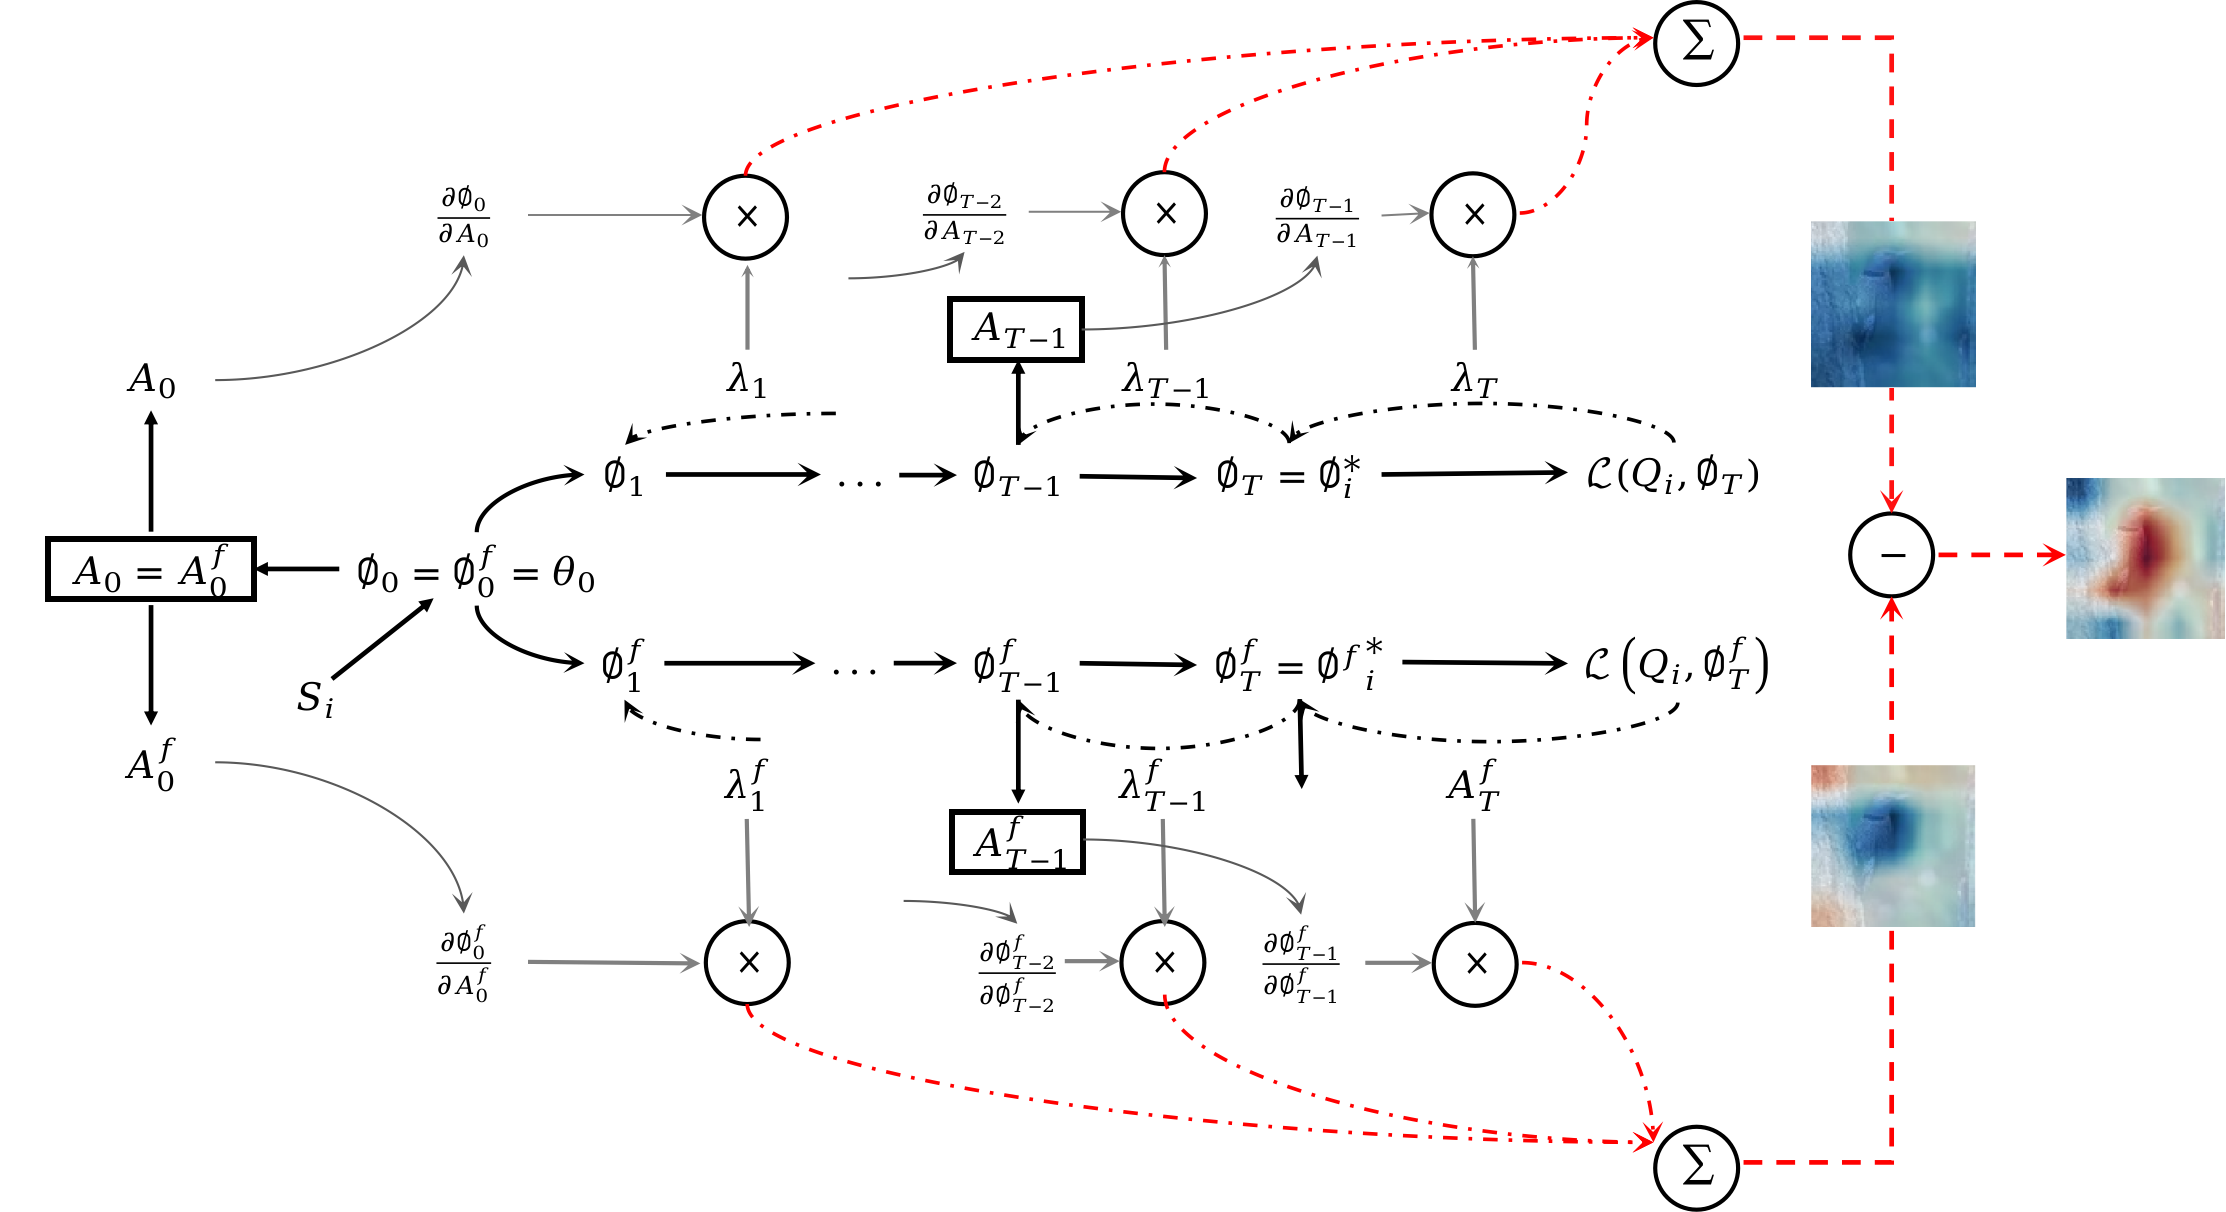
\includegraphics[width=\linewidth]{figures/fama_pipeline.png}
    \caption{\fama pipeline. Two trajectories from $S_i$ (full adaptation, top; head-only/frozen-backbone, bottom) each get one backward adjoint pass computing $\{\lambda_t\}$; at every step $\lambda_t$ is projected onto the local feature map $A_{t-1}$ (Grad-CAM style), the $T$ local maps are accumulated per branch, and the two branch maps are subtracted into $\Phi_{\mathrm{FAMA}}$.}
    \label{fig:pipeline}
\end{figure}

\paragraph{Trajectory expansion.}
One inner-loop step $\phi_t=\phi_{t-1}-\alpha\nabla_\phi\mathcal{L}(\phi_{t-1},S_i)$ has Jacobian
\begin{equation}
    \frac{\partial\phi_t}{\partial\phi_{t-1}} = I-\alpha H_{t-1},\qquad H_{t-1}:=\nabla^2_\phi\mathcal{L}(\phi_{t-1},S_i).
    \label{eq:step_jacobian}
\end{equation}
Since $S_i$ is also a shared \emph{input} to every step of \Cref{eq:inner_loop}, the chain rule sums its contribution over all $T$ steps:
\begin{equation}
    \frac{\partial\mathcal{L}(Q_i,\phi_T)}{\partial S_i} = -\sum_{t=1}^{T}\alpha\,\lambda_t\cdot\frac{\partial^2\mathcal{L}(\phi_{t-1},S_i)}{\partial\phi_{t-1}\partial S_i},\quad
    \lambda_t := \frac{\partial\mathcal{L}(Q_i,\phi_T)}{\partial\phi_t}.
    \label{eq:trajectory_expansion}
\end{equation}
Computing every $\lambda_t$ by literally unrolling and multiplying the $P\times P$ step-Jacobians of \Cref{eq:step_jacobian} is exactly the intractable BPTT case above.

\paragraph{Adjoint recursion.}
Instead, we treat $\{\lambda_t\}$ as the discrete-time adjoint (co-state) of Pontryagin's maximum principle~\cite{pontryagin1962mathematical}: initialized at the trajectory endpoint and propagated \emph{backward} one Hessian-vector product (HVP) at a time,
\begin{equation}
    \lambda_T := \mathbb{E}_{Q_i}\!\big[\nabla_\phi\mathcal{L}(Q_i,\phi_T)\big],\quad
    \lambda_{t-1} = \lambda_t - \alpha H_{t-1}\lambda_t.
    \label{eq:adjoint_recursion}
\end{equation}
We prove by backward induction (supplementary) that this recursion computes $\lambda_t=\partial\mathbb{E}_{Q_i}[\mathcal{L}(Q_i,\phi_T)]/\partial\phi_t$ \emph{exactly} at every $t$ -- no linearization is introduced beyond \Cref{eq:inner_loop} itself, since the inner loop is already a finite-step discrete system, unlike neural-ODE adjoints that must additionally discretize a continuous one. Stability requires the standard non-expansiveness condition $\alpha\le 2/\lambda_{\max}(H_{t-1})$ (formalized in the supplementary), which the fast-adaptation regime of Assumption~\ref{asm:fast_adaptation} satisfies for typical spectra. Each HVP $H_{t-1}\lambda_t$ is evaluated with Pearlmutter's double-backward trick~\cite{pearlmutter1994fast}, $H_{t-1}\lambda_t=\nabla_{\phi_{t-1}}\langle\nabla_{\phi_{t-1}}\mathcal{L},\lambda_t\rangle$, at $\mathcal{O}(P)$ cost -- never materializing $H_{t-1}$ -- so the full backward pass over $T$ steps costs $\mathcal{O}(TP)$.

\paragraph{Local attribution and CAM projection.}
Let $A_{t-1}:=f_{\phi_{t-1}^b}(S_i)\in F$ be the feature map at step $t{-}1$. Because $A_{t-1}$ is recomputed by a different backbone state at every $t$, there is no single global feature map through which one chain rule pass could flow -- instead, at each $t$ we detach $A_{t-1}$ into a leaf variable $\tilde A_{t-1}$ (stop-gradient) and define a \emph{local} attribution
\begin{equation}
    \mathrm{Attr}_{t-1} := \frac{\partial}{\partial A_{t-1}}\Big[\lambda_t\!\cdot\!\nabla_\phi\mathcal{L}(\phi_{t-1},S_i)\Big],\ t=1,\dots,T,
    \label{eq:local_attr}
\end{equation}
which, because the backbone is formally frozen at this step, reduces to exactly the head/feature Hessian block $\partial^2\mathcal{L}/\partial\phi^h\partial A$. We turn $\mathrm{Attr}_{t-1}$ ($C\times H\times W$) into a heatmap with the standard Grad-CAM recipe~\cite{selvaraju2020grad} -- global-average-pool to channel weights $w_t^c$, weight-and-sum $A_{t-1}$, bilinearly upsample -- applied independently at every $t$, then accumulated along the trajectory:
\begin{equation}
    \Phi(x_k^S) := \sum_{t=1}^{T}\alpha\,\widehat{\mathrm{CAM}}_{t-1}(x_k^S).
    \label{eq:branch_saliency}
\end{equation}
Unlike Grad-CAM, we \emph{do not} apply ReLU: both the sign of help and the sign of harm are diagnostic here, so $\widehat{\mathrm{CAM}}_{t-1}$ keeps its sign throughout. Running this for both the full and frozen branches and subtracting isolates the part of the signal attributable to the backbone actually moving:
\begin{equation}
    \boxed{\ \PhiFama(x_k^S) := \Phi_{\mathrm{full}}(x_k^S) - \Phi_{\mathrm{freeze}}(x_k^S).\ }
    \label{eq:fama_final}
\end{equation}
$\Phi_{\mathrm{freeze}}$ is a static feature-reuse baseline (constant backbone across all $t$), so \Cref{eq:fama_final} cancels whatever the two branches would have attributed in common and keeps only the part caused by the backbone's own displacement -- the same quantity \Cref{prop:decomposition} identifies as $C_b$. Regions with $\PhiFama{>}0$ are where adaptation \emph{helped}; regions with $\PhiFama{<}0$ are where it \emph{hurt}. \Cref{alg:fama} summarizes the full computation; because the spatial upsampling in \Cref{eq:branch_saliency} assumes a convolutional feature grid, \fama as stated targets convolutional backbones (\Cref{sec:limitations}).

\begin{algorithm}[t]
\caption{\fama}
\label{alg:fama}
\begin{algorithmic}[1]
\Require $\theta_0$, task $(S_i,Q_i)$, steps $T$, rate $\alpha$
\Ensure adaptation gain $\Delta M$, attribution map $\PhiFama$
\State $m \gets$ head mask of $\theta_0$ (last param.\ block)
\State roll out $\{\phi_t\}_{t=0}^T$ via \Cref{eq:inner_loop}; $\{\phi_t^f\}_{t=0}^T$ likewise but reset backbone params to $\theta_0^b$ after every step ($m$)
\State $\Delta M \gets$ bootstrap estimate of \Cref{eq:adaptation_gain} over $Q_i$
\For{branch $X \in \{\phi, \phi^f\}$}
    \State $\lambda_T \gets \mathbb{E}_{Q_i}[\nabla_\phi \mathcal{L}(Q_i, X_T)]$ \Comment{bootstrap}
    \For{$t = T, \dots, 1$}
        \State $\lambda_{t-1} \gets \lambda_t - \alpha\cdot\mathrm{HVP}(X_{t-1}, \lambda_t, S_i)$ \Comment{Eq.~\eqref{eq:adjoint_recursion}, Pearlmutter}
    \EndFor
    \State $\Phi_X \gets 0$
    \For{$t = 1, \dots, T$}
        \State $\Phi_X \mathrel{+}= \alpha \cdot \mathrm{GradCAM}(X_{t-1}, \lambda_t, S_i)$ \Comment{Eqs.~\eqref{eq:local_attr}--\eqref{eq:branch_saliency}, no ReLU}
    \EndFor
\EndFor
\State \Return $\Delta M$, $\ \PhiFama \gets \Phi_{\phi} - \Phi_{\phi^f}$
\end{algorithmic}
\end{algorithm}

\paragraph{Practical overhead.} \Cref{alg:fama} makes the concrete cost relative to a single Grad-CAM call (one forward pass, one backward pass, evaluated once at $\phi_T$) explicit: per branch, $T$ inner-loop steps to roll out the trajectory, $T$ Hessian-vector products for the adjoint recursion (each a small constant number of extra forward/backward passes via Pearlmutter's trick~\cite{pearlmutter1994fast}), and $T$ local Grad-CAM projections -- for both the full and frozen branch. Every one of these is a fixed-size pass through the same backbone; none grows with the parameter count $P$. So the overhead over one static Grad-CAM call is $\Theta(T)$ backbone evaluations with a small constant factor, not the quadratic-in-$P$ blowup literal backpropagation-through-time would incur -- exactly the trade the adjoint recursion makes. We have not yet measured this as wall-clock time against a Grad-CAM/TL-XML/TracIn baseline (\Cref{sec:limitations}); the count above is architectural, derived directly from \Cref{alg:fama}, not measured.
